\subsection{Effect of Memory Bandwidth Throttling}

In this subsection, we examine the CNN workload's memory bandwidth
sensitivity and the effect of memory bandwidth throttling in providing
isolation. For the experiments, we use MemGuard\cite{Yun2013}, a Linux
kernel module that can limit the amount of memory bandwidth each core
receives. MemGuard
operates periodically, at a 1 ms interval, and uses hardware
performance counters to throttle cores, if they exceed their given
bandwidth budgets within each regulation period (i.e., 1 ms), by
scheduling high-priority idle kernel threads until the next period begins.


In the first experiment, we measure the performance of the CNN model
on a single core, first w/o using MemGuard and then w/
using MemGuard while varying the core's bandwidth throttling parameter
from 500 MB/s down to 100 MB/s.

\begin{figure}[h]
  \centering
  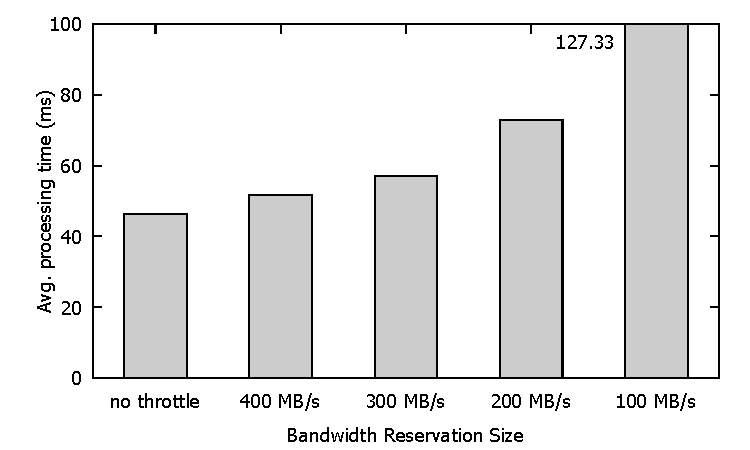
\includegraphics[width=.45\textwidth]{figs/memguard_multicore}
  \caption{Memory bandwidth sensitivity of the CNN control loop.}
  \label{fig:memguard_multicore}
\end{figure}

Figure \ref{fig:memguard_multicore} shows the results. When the core
executing the CNN model is throttled at 400 MB/s or more, the performance
of the model is largely the same as the non-throttled case. However, as
we decrease the assigned memory bandwidth below 300 MB/s, we start to
observe noticeable decreases in the model's performance. In other
words, the CNN model is sensitive to memory bandwidth and it
requires 400 MB/s or more bandwidth to ensure ideal performance.

In the next experiment, we repeat the experiment in
Section~\ref{sec:eval-memhog}---i.e., co-scheduling memory intensive
synthetic tasks---but this time we
throttle the cores of the co-runners using MemGuard and vary their
memory bandwidth budgets to see their impact on the CNN model's 
performance.

\begin{figure}[h]
  \centering
  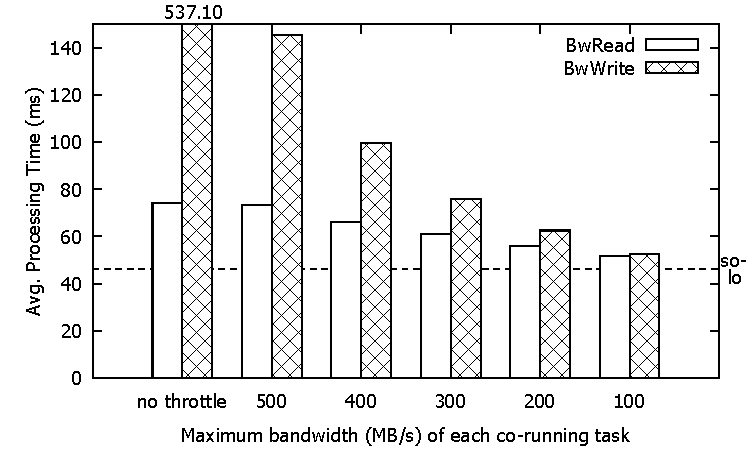
\includegraphics[width=.45\textwidth]{figs/memguard_bandwidth}
  \caption{Effect of throttling three memory intensive co-runners.} 
  \label{fig:memguard_bandwidth}
\end{figure}

Figures \ref{fig:memguard_bandwidth} shows the results.
As can clearly be seen in the figure, limiting the co-runners's memory
bandwidth is effective in protecting the CNN model's performance for
BwRead and BwWrite co-runners. The benefits are especially more
pronounced in case of BwWrite co-runners as, when we throttle them more, the
CNN's performance quickly improves.

%% Note that, in case of BwWrite co-runners, we assign half the
%% bandwidth budget because MemGuard only accounts for L2 refills
%% but not write-backs, which effectively allows twice the allocated
%% memory bandwidth budget.

In summary, we find that the CNN inferencing workload is sensitive to
memory bandwidth and that memory bandwidth throttling is effective in
improving the performance isolation of the CNN workload.

%% \begin{figure}[h]
%%   \centering
%%   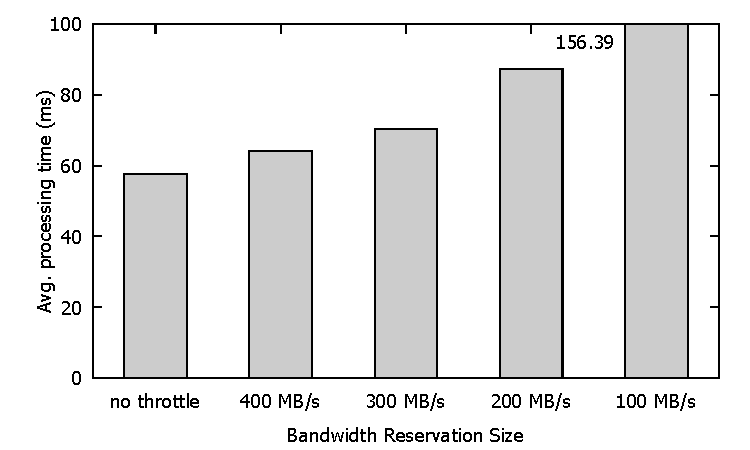
\includegraphics[width=.45\textwidth]{figs/memguard_multimodel}
%%   \caption{Timing impact of co-scheduling multiple DNNs when memory
%% bandwidth throttling is enabled. }
%%   \label{fig:memguard_multimodel}
%% \end{figure}

%% We also test the effects of memory bandwidth throttling in the case 
%% of multiple models running concurrently on the Pi 3 by rerunning the 
%% 4Nx1C experiment. We use the same memory bandwidth reservation sizes 
%% from the previous experiment. The results can be seen in Figure
%% \ref{fig:memguard_multimodel}. Once again, the performance of the 
%% models are affected by the amount of memory bandwidth that is 
%% available to the Pi 3's cores during each period, meaning that they 
%% are all memory dependent.

%% \begin{figure}[h]
%%   \centering
%%   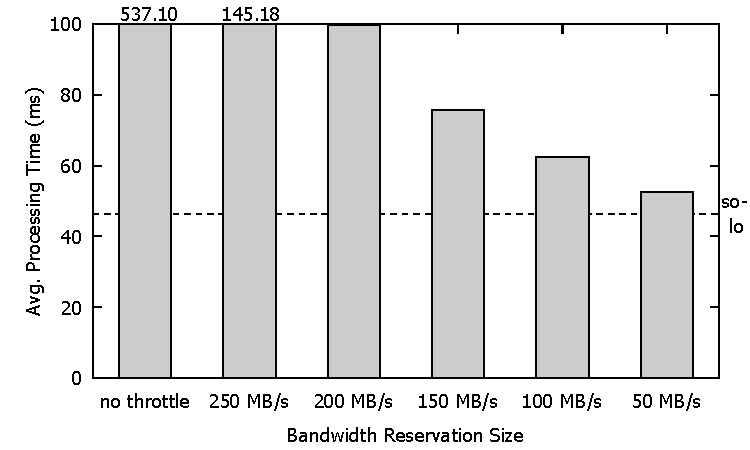
\includegraphics[width=.45\textwidth]{figs/memguard_bwwrite}
%%   \caption{Timing impact of co-scheduling memory intensive write
%% co-runners when memory bandwidth throttling is enabled. }
%%   \label{fig:memguard_bwwrite}
%% \end{figure}


%% In the case of one co-runner, the performance of the model remains 
%% constant even as the reservation sizes are decreased, however, it 
%% still improves compared to when throttling wasn't enabled. 
%% In both cases, when the co-runners were given a minimal reservation size,
%% the performance of the model was much closer to its solo execution time.
%% This is especially noteworthy when write co-runners were present, as the 
%% model didn't suffer the same 11.6X slowdown that was seen without
%% bandwidth throttling enabled. 
%% %% When memory intensive Bandwidth benchmarks were present, model performance
%% %% improved, to a notable extent, through the use of memory bandwidth 
%% %% throttling on the co-runners. 
%% Since this would not be the case if the 
%% model was memory insensitive, we find that the model is memory 
%% dependent in the presence of co-runners.

%% Based on all of the memory bandwidth throttling experiments 
%% performed, it is evident that the shared DRAM memory is important for
%% the DNN model. When a single model was run, its 
%% performance decreased as less memory bandwidth was 
%% made available to it. Furthermore, when the bandwidths of memory 
%% intensive read and write co-runners were limited, the performance of 
%% the model improved. As such, we conclude that the model is dependent on the 
%% shared DRAM memory.
